%%%%%%%%%%%%%%%%%%%%%%%%%%%%%%%%%%%%%%%%%%%%%%%%%%%%%%%%%%%%%%%%%%%%%%%%%%%%%%
%% AMS-LaTeX Paper
%%%%%%%%%%%%%%%%%%%%%%%%%%%%%%%%%%%%%%%%%%%%%%%%%%%%%%%%%%%%%%%%%%%%%%%%%%%%%%
\documentclass[12pt,leqno]{amsart}
\pdfoutput=1
\usepackage{amsmath, amssymb, amsthm}
% \usepackage{rsfso}
\usepackage[svgnames]{xcolor}
\usepackage{tikz}
\usetikzlibrary{arrows,cd}
\tikzset{>=latex}
\usepackage{mathtools}
\usepackage[alwaysadjust]{paralist}
\usepackage[alphabetic]{amsrefs}
\usepackage[T1]{fontenc}
\usepackage{mathptmx}
\usepackage{microtype}
\linespread{1.06}
\usepackage[colorlinks = true,
  linkcolor  = DarkBlue,
  urlcolor   = DarkRed,
  citecolor  = DarkGreen]{hyperref}
\hypersetup{
  pdftitle={The simplicial complexes package for Macaulay2},
  pdfauthor={Ben Hersey, Gregory G. Smith, and Alexandre Zotine}
}
%% --Extras------------------------------------------------------------------
\usepackage{caption}
\usepackage{subcaption}
%% --LAYOUT-------------------------------------------------------------------
\usepackage[centering, includeheadfoot, hmargin=1.0in, tmargin=1.0in,
  bmargin=1in, headheight=6pt]{geometry}
%% --DISPLAY CODE------------------------------------------------------------
\usepackage{listings}
\lstset{
  basicstyle=\ttfamily,
  mathescape
}
%% --OTHER ENVIRONMENTS-------------------------------------------------------
\newtheorem{lemma}{Lemma}[section]
\newtheorem{theorem}[lemma]{Theorem}
\newtheorem{maintheorem}{Theorem}
\newtheorem{corollary}[lemma]{Corollary}
\newtheorem{proposition}[lemma]{Proposition}
\theoremstyle{definition}
\newtheorem{definition}[lemma]{Definition}
\newtheorem{remark}[lemma]{Remark}
\newtheorem{examplex}[lemma]{Example}
\newenvironment{example}
{\pushQED{\qed}\renewcommand{\qedsymbol}{$\diamond$}\examplex}
{\popQED\endexamplex}
\newtheorem{question}[lemma]{Question}
\renewcommand{\theequation}{\arabic{section}.\arabic{lemma}.\arabic{equation}}
\renewcommand{\thetable}{\arabic{section}.\arabic{lemma}.\arabic{equation}}
\renewcommand{\themaintheorem}{\Alph{maintheorem}}

%% --MATH---------------------------------------------------------------------
\newcommand{\PP}{\ensuremath{\mathbb{P}}}
%% Operators
\DeclareMathOperator{\Hom}{Hom}
\DeclareMathOperator{\Proj}{Proj}
\DeclareMathOperator{\Spec}{Spec}
\DeclareUnicodeCharacter{0393}{\Gamma}
\DeclareUnicodeCharacter{0394}{\Delta}
\DeclareUnicodeCharacter{22C8}{\bowtie}
%\DeclareUnicodeCharacter{29D3}{}
%\DeclareUnicodeCharacter{}


%%%%%%%%%%%%%%%%%%%%%%%%%%%%%%%%%%%%%%%%%%%%%%%%%%%%%%%%%%%%%%%%%%%%%%%%%%%%%%
\begin{document}

\title[Simplicial Complexes]{The simplicial complexes package for Macaulay2}
\author[B.~Hersey]{Ben Hersey}
\address{Ben Hersey: Department of Mathematics and Statistics, Queen's University, Kingston, Ontario, K7L 3N6;
  {\normalfont \texttt{b.hersey@queensu.ca}}}

\author[G.G.~Smith]{Gregory G.{} Smith}
\address{Gregory G.{} Smith: Department of Mathematics and Statistics, Queen's
  University, Kingston, Ontario, K7L 3N6, Canada; {\normalfont
    \texttt{ggsmith@mast.queensu.ca}}}

\author[A.~Zotine]{Alexandre Zotine}
\address{Alexandre Zotine: Department of Mathematics and Statistics, Queen's University, Kingston, Ontario, K7L 3N6;
  {\normalfont \texttt{18az45@queensu.ca}}}

\thanks{todo grant stuff \emph{Mathematics Subject Classification}. todo}
\date{\today}

\begin{abstract}
  This article demonstrates some of the updated features of the \texttt{SimplicialComplexes} package in \emph{Macaulay2}. todo
\end{abstract}

\maketitle


%%%%%%%%%%%%%%%%%%%%%%%%%%%%%%%%%%%%%%%%%%%%%%%%%%%%%%%%%%%%%%%%%%%%%%%%%%%%%%
\addcontentsline{toc}{section}{Overview}
\addtocounter{section}{1}
\addtocounter{lemma}{-1}

\noindent

%%%%%%%%%%%%%%%%%%%%%%%%%%%%%%%%%%%%%%%%%%%%%%%%%%%%%%%%%%%%%%%%%%%%%%%%%%%%%%
\section{Combinatorial Topology}

Lutz has provided a database enumerating all of the 2 and 3-manifolds having 10 or less vertices. We have implemented these databases into the package---however we have excluded the database of 3-manifolds with 10 vertices, due to the large number of examples causing long loading times.
\begin{example}\label{example of using database}
  These databases can be used to find nice testbeds of examples: for instance, we can search for simplicial maps
  %
  \begin{lstlisting}[basicstyle={\ttfamily \scriptsize}, xleftmargin=-23pt]
    i2 : R = ZZ[a..i];
    i3 : S = ZZ[x_0..x_6];
    i4 : $Γ$ = smallManifold(2,7,1,S);
    i5 : maplist = flatten for i to 2 list (
         for j in subsets(toList(R_0..R_8),7) list (
             phi := map(smallManifold(3,9,i,R),$Γ$,j);
             if isWellDefined phi then phi else continue
             )
         );
    i6 : maplist_0
    o6 = | a b e f g h i |
  \end{lstlisting}
  %
  By construction, all of these maps should be inclusions.
  %
  \begin{lstlisting}[basicstyle={\ttfamily \scriptsize}, xleftmargin=-23pt]
    i7 : isInjective\maplist
    o7 = {true, true, true, true, true, true}
    o7 : List
  \end{lstlisting}
  %
\end{example}
The database also contains many triangulations of various interesting surfaces, such as the torus, Klein bottle, and real projective plane. Here are the smallest indices (and hence minimal triangulations of) these surfaces in the database
\begin{example}\label{example of using database}
  %
  \begin{lstlisting}[basicstyle={\ttfamily \scriptsize}, xleftmargin=-23pt]
    i8 : Torus = smallManifold(2, 7, 6, R);
    i9 : KleinBottle = smallManifold(2, 8, 12, R);
    i10 : RP2 = smallManifold(2, 6, 1, R);
  \end{lstlisting}
  %
  We can check that these are the right surfaces by computing their homology. Theorems 6.2, 6.3, and 6.4 from Munkres confirm that they match \cite{Munkres}.
  %
  \begin{lstlisting}[basicstyle={\ttfamily \scriptsize}, xleftmargin=-23pt]
    i11 : for i to 2 list prune HH_i Torus
                2    1
    o11 = {0, ZZ , ZZ }
    o11 : List
    i12 : for i to 2 list prune HH_i KleinBottle
    o12 = {0, cokernel | 2 |, 0}
                       | 0 |
    o12 : List
    i13 : for i to 2 list prune HH_i RP2
    o13 = {0, cokernel | 2 |, 0}
    o13 : List
  \end{lstlisting}
  We can explicitly identify the generators of the homology for the torus.
  \begin{lstlisting}[basicstyle={\ttfamily \scriptsize}, xleftmargin=-23pt]
    i0 : TODO. Ben's code
  \end{lstlisting}
  %
\end{example}

%%%%%%%%%%%%%%%%%%%%%%%%%%%%%%%%%%%%%%%%%%%%%%%%%%%%%%%%%%%%%%%%%%%%%%%%%%%%%%
\section{Stanley-Reisner Theory}

\noindent
Let $\Delta$ be an abstract simplicial complex with vertex set $V = \{v_0,v_1,...,v_{n-1}\}$, let $k$ be a commutative ring, and let $S = k[x_0,x_1,...,x_n]$. The \textbf{Stanley-Reisner ideal}, or \textbf{facet ideal} of $\Delta$ is defined to be square-free monomial ideal
%
\begin{displaymath}
  I_\Delta := \left( \prod_{j=1}^k x_{i_j} \ \bigg\vert \ \{ v_{i_1},v_{i_2},...,v_{i_k} \} \not \subset \Delta \right) \subset S,
\end{displaymath}
%
and the \textbf{Stanley-Reisner ring} corresponding to $\Delta$ is $k[\Delta] = S/I_\Delta$. This correspondence between simplicial complexes and square-free monomial ideals is one-to-one. Stanley-Reisner theory connects homological properties of $k[\Delta]$ to combinatorial and topological properties of $\Delta$. A survey of results can be found in \cite{BH, Stanley, MS}.

If $I = (m_1,...,m_q) \subset S$ is a monomial ideal, with minimal generators $m_i = \displaystyle \prod x_j^{a_{i_j}}$, then the \textbf{Alexander dual} of $I$ is defined to be $\displaystyle I^* := \bigcap_{i=1}^q\hspace{2pt} (x_0^{a_{i_1}},\ x_1^{a_{i_2}},...,\ x_{n-1}^{a_{i_{n-1}}})$. If $I = I_\Delta$ for some simplicial complex $\Delta$, then $I^*$ is also a square-free monomial ideal and is the Stanley-Reisner ideal of a simplicial complex $\Delta^*$, which we call the \textbf{Alexander dual} complex to $\Delta$. There is also a combinatorial description of $\Delta^*$, given by $\Delta^* = \{ F \subset V \ | \ V \setminus F \not \in \Delta \}$. One of the attractive features of Alexander duality is the relationship between the cohomology of $\Delta$ and the homology of $\Delta^*$. More specifically, if $\Delta$ is a simplicial complex on $n$ vertices, then $    \widetilde{H}_{i-1}(\Delta^*) = \widetilde{H}^{n-2-i}(\Delta)$ for all $i \in \mathbb Z$, see \cite[Theorem 5.6]{MS}.
%
% \begin{theorem}[Alexander duality for simplicial complexes]\label{Combinatorial Alexander duality}
%   Let $\Delta$ be a simplicial complex with vertex set $V = \{v_1,v_2,..,v_n \}$. Then
%   %
%   \begin{displaymath}
%     \widetilde{H}_{i-1}(\Delta^*) = \widetilde{H}^{n-2-i}(\Delta)
%   \end{displaymath}
%   %
%   for all $i \in \mathbb Z$.
% \end{theorem}
%
\begin{example}\label{Example: Stanley-Reisner ideal and Alexander duality for the bowtie complex}
  Consider the simplicial complex $\bowtie$, depicted in Figure \ref{the figure-8 and its dual}
  %
  \begin{figure}[h]
    \begin{subfigure}{0.3\textwidth}
      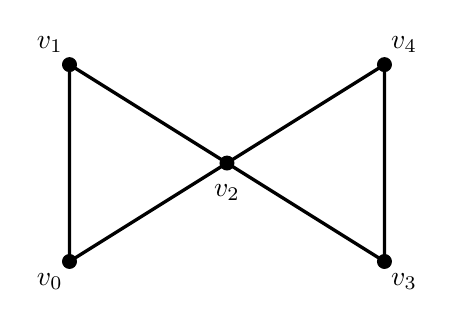
\begin{tikzpicture}[scale = .5]
        % \filldraw[gray!10] (0,0) -- (0,5) -- (4,2.5) -- cycle;
        \draw[-,very thick] (0,0) -- (0,5) -- (4,2.5) -- cycle;
        % \filldraw[gray!10] (8,0) -- (8,5) -- (4,2.5) -- cycle;
        \draw[-,very thick] (8,0) -- (8,5) -- (4,2.5) -- cycle;
        \filldraw (0,0) circle (5pt);
        \filldraw (0,5) circle (5pt);
        \filldraw (4,2.5) circle (5pt);
        \filldraw (8,0) circle (5pt);
        \filldraw (8,5) circle (5pt);
        \node at (-.5,-.5) {$v_0$};
        \node at (-.5,5.5) {$v_1$};
        \node at (4,1.75) {$v_2$};
        \node at (8.5,-.5) {$v_3$};
        \node at (8.5,5.5) {$v_4$};
        % \node at (-2.5,2.5) {\huge $\Delta \hspace{5pt} = $};
      \end{tikzpicture}
%      \caption{The simplicial complex $\Delta$}\label{figure-8 complex}
    \end{subfigure}
    \hspace{50pt}
    \begin{subfigure}{0.3\textwidth}
      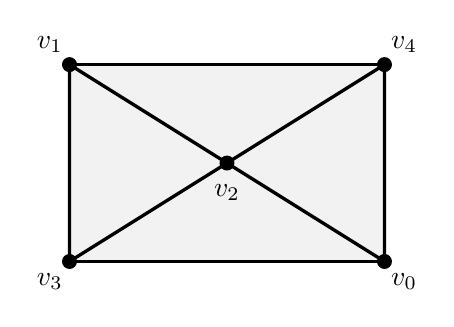
\begin{tikzpicture}[scale = .5]
        \filldraw[gray!10] (0,0) -- (0,5) -- (4,2.5) -- cycle;
        \filldraw[gray!10] (8,0) -- (8,5) -- (4,2.5) -- cycle;
        \filldraw[gray!10] (0,0) -- (8,0) -- (4,2.5) -- cycle;
        \filldraw[gray!10] (0,5) -- (8,5) -- (4,2.5) -- cycle;
        \draw[-,very thick] (0,0) -- (0,5) -- (4,2.5) -- cycle;
        \draw[-,very thick] (8,0) -- (8,5) -- (4,2.5) -- cycle;
        \draw[-,very thick] (0,5) -- (8,5);
        \draw[-,very thick] (0,0) -- (8,0);
        \filldraw (0,0) circle (5pt);
        \filldraw (0,5) circle (5pt);
        \filldraw (4,2.5) circle (5pt);
        \filldraw (8,0) circle (5pt);
        \filldraw (8,5) circle (5pt);
        \node at (-.5,-.5) {$v_3$};
        \node at (-.5,5.5) {$v_1$};
        \node at (4,1.75) {$v_2$};
        \node at (8.5,-.5) {$v_0$};
        \node at (8.5,5.5) {$v_4$};
        % \node at (-2.5,2.5) {\huge $\Delta^* = $};
      \end{tikzpicture}
%      \caption{The Alexandual Dual of $\Delta$}
    \end{subfigure}
    \caption{The simplicial complex $\bowtie$ (left) and its Alexander dual $\bowtie^*$ (right).}\label{the figure-8 and its dual}
  \end{figure}
  %
  The Stanley-Reisner ideal of $\bowtie$ is $I_{\bowtie} = (x_0x_1x_2,\ x_0x_3,\ x_1x_3,\ x_0x_4,\ x_1x_4,\ x_2x_3x_4)$. We can exhibit the correspondence between $\Delta$ and $I_\Delta$ using the methods \texttt{simplicialComplex} and \texttt{ideal}.
  %
  \begin{lstlisting}[basicstyle={\ttfamily \scriptsize}, xleftmargin=-23pt]
    i28 : S = QQ[x_0..x_4];
    i29 : I$⋈$ = monomialIdeal(x_0*x_1*x_2,x_0*x_3,x_1*x_3,x_0*x_4,x_1*x_4,x_2*x_3*x_4);
    o29 : MonomialIdeal of S
    i30 : $⋈$ = simplicialComplex I$⋈$
    o30 = simplicialComplex | x_3x_4 x_2x_4 x_2x_3 x_1x_2 x_0x_2 x_0x_1 |
    o30 : SimplicialComplex
    i31 : I$⋈$ == ideal $⋈$
    o31 = true
  \end{lstlisting}
  %
  We can use the \texttt{dual} method to compute the Alexander dual of $\Delta$.
  % 
\begin{lstlisting}[basicstyle={\ttfamily \scriptsize}, xleftmargin=-23pt]
    i133 : dual $⋈$
    o133 = simplicialComplex | x_1x_2x_4 x_0x_2x_4 x_1x_2x_3 x_0x_2x_3 |
    o133 : SimplicialComplex
\end{lstlisting}
  %
  which is the simplicial complex
    % 
  By the definition of the Alexander dual, we know that $(I_\Delta)^* = I_{\Delta^*}$. We can verify this directly.
  % 
\begin{lstlisting}[basicstyle={\ttfamily \scriptsize}, xleftmargin=-23pt]
    i134 : dual(monomialIdeal $Δ$) == monomialIdeal dual $Δ$
    o134 = true
\end{lstlisting}
  % 
  We can also verify the combinatorial description of $\Delta^*$ by showing that the minimal generators of $I_\Delta$ correspond the complements of the facets of $\Delta^*$,
  % 
\begin{lstlisting}[basicstyle={\ttfamily \scriptsize}, xleftmargin=-23pt]
    i140 : dualFacets = first entries facets dual $Δ$
    o140 = {x x x , x x x , x x x , x x x }
             1 2 4   0 2 4   1 2 3   0 2 3
    o140 : List
    i141 : sort first entries gens I$Δ$ == sort for F in dualFacets list(
               product for v in vertices $Δ$ list(
                   if member(v, support F) then continue else v)
                   )
               )
    o141 = true
\end{lstlisting}
  % 
  Finally, we exhibit the isomorphisms between the cohomology of $\Delta$ and the homology of $\Delta^*$.
  % 
\begin{lstlisting}[basicstyle={\ttfamily \scriptsize}, xleftmargin=-23pt]
    i94 : all(-1..5, i -> all(-1..5, i -> prune HH^(3-i) $Δ$ == prune HH_(i-1) dual $Δ$)
    o94 = true
\end{lstlisting}  
\end{example}
%
For a face $F \in \Delta$, we define the \textbf{link} of $F$, is the subcomplex of $\Delta$ defined by
%
\begin{displaymath}
  \mathrm{link}_\Delta(F) := \{ G \in \Delta \ | \ F \cup G \in \Delta \ \text{ and } \ F \cap G = \varnothing \}.
\end{displaymath}
%
We can now exhibit a more substantive result of Stanley-Reisner theory, which is the ``dual version'' of Hochster's formula, see \cite[Corollary 1.40]{MS}. This formula allows us to compute the multigraded Betti numbers of $I_\Delta$, which are defined to be $\beta_{i,m}(I_\Delta) = \big( \mathrm{Tor}_i^S(I_\Delta, k) \big)_m$. For a subset $F \subset V$, we will use the notation $\beta_{i,F}$ to refer to the betti number in homological degree $i$ and multidegree $(a_1,...,a_n) \in \mathbb Z^n$, where $a_i = 1$ if $v_i \in F$ and $a_i = 0$ otherwise.
%
\begin{theorem}[Hochster's Formula, dual version]
  Let $\Delta$ be a simplicial complex with vertex set $V = \{ v_0,v_1,...,v_{n-1} \}$. The nonzero multigraded Betti numbers of $I_\Delta$ and $S/I_\Delta$ lie in squarefree degrees. Moreover, if $F \subset V$, then
  %
  \begin{displaymath}
    \beta_{i,F} (I_\Delta) = \beta_{i+1,F} (S/I_\Delta) = \dim_k\Big(\widetilde H_{i-1} \big( \mathrm{link}_{\Delta^*}(V \setminus F)\; ; \; k \big) \Big).
  \end{displaymath}
\end{theorem}
%
\begin{example}
  In Example \ref{Stanley-Reisner ideal and Alexander duality}, we computed the Alexander dual of the figure-8 complex. We can use the \texttt{link} method to compute the links of various faces. For example, we compute the link of the central vertex $v_2$, whose link is a square.
  % 
\begin{lstlisting}[basicstyle={\ttfamily \scriptsize}, xleftmargin=-23pt]
    i27 : link(dual $Δ$, x_2)
    o27 = simplicialComplex | x_1x_4 x_0x_4 x_1x_3 x_0x_3 |
    o27 : SimplicialComplex
\end{lstlisting}
  %
  We can also construct a function that computes the multigraded betti numbers $\beta_{i,F}(S/I_\Delta)$.
  %
\begin{lstlisting}[basicstyle={\ttfamily \scriptsize}, xleftmargin=-23pt]
    hochster = (i, m) -> (
        G := product select(vertices $Δ$, v -> not member(v, support m));
        rank (homology link(dual $Δ$, G_S))_i
        )
\end{lstlisting}
  %
  Since we have a bound on the nonzero betti numbers of $I_\Delta$, we can collect them into a matrix
  %
\begin{lstlisting}[basicstyle={\ttfamily \scriptsize}, xleftmargin=-23pt]
    i94 : V = vertices $Δ$;
    i95 : squarefreeMonomials = unique sort apply(remove(subsets V, 0), m -> lcm m);
    i96 : matrix for i to length res I$Δ$ - 1 list (
              for F in squarefreeMonomials list hochster(i-1,F)
              )
    o96 = | 0 0 0 0 0 0 0 1 1 0 1 1 0 0 0 1 0 0 0 0 0 0 0 0 1 0 0 0 0 0 0 |
          | 0 0 0 0 0 0 0 0 0 0 0 0 0 0 0 0 1 1 0 0 1 0 0 1 0 1 1 0 1 1 0 |
          | 0 0 0 0 0 0 0 0 0 0 0 0 0 0 0 0 0 0 0 0 0 0 0 0 0 0 0 1 0 0 2 |
                   3        31
    o96 : Matrix ZZ  <--- ZZ
\end{lstlisting}
  % 
  where the row are indexed by the homological degree (starting at $0$), and the columns are indexed by the squarefree multidegrees.
\end{example}
% 
We say that a simplicial complex $\Delta$ is \textbf{pure} if all of the facets of $\Delta$ have the same dimension. We say that \textbf{shellable} if we can order the facets $F_1,...,F_m$ of $\Delta$ so that $\langle F_i \rangle \cap \langle F_1,F_2,...,F_{i-1} \rangle$ is a pure, codimension $1$, simplicial complex. We say that a $\Delta$ is \textbf{Cohen-Macaulay} if $k[\Delta]$ is a Cohen-Macaulay ring. It is known that every shellable simplicial complex is Cohen-Macaulay \cite[Theorem 5.1.13]{BH} and every Cohen-Macaulay simplicial complex is pure \cite[Corollary 5.1.5]{BH}.

% The figure-8 complex from example \ref{Example: Stanley-Reisner ideal and Alexander duality for the bowtie complex} is pure, shellable, and Cohen-Macaulay. Verifying shellability of a simplicial complex can be done using the \texttt{SimplicialDecomposability} package in \texttt{Macaulay2}, \cite{Cook}.

For Stanley-Reisner rings, we can use the combinatorics of $\Delta$ to determine if $k[\Delta]$ is a Cohen-Macaulay ring. Specifically, $k[\Delta]$ is Cohen-Macaulay if an only if $\widetilde H_i(\mathrm{link}_\Delta(F);k) = 0$ for all $F \in \Delta$ and $i < \dim \hspace{2pt} \mathrm{Link}_\Delta(F)$, see \cite[Corollary 5.3.9]{BH}. We can also relate the Cohen-Macaulay property to the $h$-vector of $\Delta$. We can write the Hilbert series of $k[\Delta]$ as a rational function
%
\begin{displaymath}
  \sum \dim \hspace{2pt} k[\Delta]_i \hspace{2pt} t^i = \frac {h_0 + h_1t + \cdots h_k t^k}{(1-t)^d}
\end{displaymath}
%
where $d = \dim \Delta + 1$, and $0 \leq k \leq d$ is such that $h_k \not = 0$. If $\Delta$ is a $d$-dimensional Cohen-Macaulay complex with $n$ vertices, then \cite[Lemma 5.1.10]{BH} proves that
%
\begin{displaymath}
  0 \leq h_i \leq \binom{n-d+i}{i}
\end{displaymath}
%
for $i = 0,1,...,d+1$. We can also compute the $h$-vector using the combinatorics of $\Delta$. Specifically, if $\Delta$ is a $d$-dimensional simplicial complex, then \cite[Lemma 5.18]{BH} tells us that
%
\begin{displaymath}
  h_j = \sum_{i=0}^j (-1)^{j-1} \binom{d+1-i}{j-1}f_{i-1}
\end{displaymath}
%
for $j = 0,1,...,d+1$.
%
\begin{example}\label{Example: Shellability, the Cohen-Macaulay property, and the h-vector}
  The figure $8$ complex introduced in example \ref{Example: Stanley-Reisner ideal and Alexander duality for the bowtie complex} is Shellable and Cohen-Macaulay. We can verify the Cohen-Macaulay property using \cite[Corollary 5.3.9]{BH}.
  % 
\begin{lstlisting}[basicstyle={\ttfamily \scriptsize}, xleftmargin=-23pt]
    i43 : faceList = flatten for i from -1 to dim $Δ$ list (faces $Δ$)#i
    o43 = {1, x , x , x , x , x , x x , x x , x x , x x , x x , x x }
               0   1   2   3   4   0 1   0 2   1 2   2 3   2 4   3 4
    o43 : List
    i44 : all(faceList, F -> all(0..dim(link($⋈$,F))-1, i -> HH_i link($Δ$,F) == 0))
    o44 = true
\end{lstlisting}
  % 
  This simplicial complex is also shellable, but this package does not provide a method for determining this quality. However, such a method is available in the \texttt{SimplicialDecomposability} package in \texttt{Macaulay2}, see \cite{Cook}.

  We instead consider the ``bowtie'' simplicial complex, which we can obtain by filling in the facets of the $2$-faces of the figure $8$ simplicial complex, see Figure 
\end{example}

%





% \begin{figure}[h]
%   \begin{tikzpicture}[scale = .5]
%     \filldraw[gray!10] (0,0) -- (0,5) -- (4,2.5) -- cycle;
%     \draw[-,very thick] (0,0) -- (0,5) -- (4,2.5) -- cycle;
%     \filldraw[gray!10] (8,0) -- (8,5) -- (4,2.5) -- cycle;
%     \draw[-,very thick] (8,0) -- (8,5) -- (4,2.5) -- cycle;
%     \filldraw (0,0) circle (5pt);
%     \filldraw (0,5) circle (5pt);
%     \filldraw (4,2.5) circle (5pt);
%     \filldraw (8,0) circle (5pt);
%     \filldraw (8,5) circle (5pt);
%     \node at (-.5,-.5) {$v_0$};
%     \node at (-.5,5.5) {$v_1$};
%     \node at (4,1.75) {$v_2$};
%     \node at (8.5,-.5) {$v_3$};
%     \node at (8.5,5.5) {$v_4$};
%     % \node at (-2.5,2.5) {\huge $\Delta \hspace{5pt} = $};
%   \end{tikzpicture}
%   \caption{The bowtie complex}\label{bowtie figure}
% \end{figure}



%
%%%%%%%%%%%%%%%%%%%%%%%%%%%%%%%%%%%%%%%%%%%%%%%%%%%%%%%%%%%%%%%%%%%%%%%%%%%%%%
\section{Resolutions Of Monomial Ideals}



%%%%%%%%%%%%%%%%%%%%%%%%%%%%%%%%%%%%%%%%%%%%%%%%%%%%%%%%%%%%%%%%%%%%%%%%%%%%%%
\subsection*{Acknowledgements}
We thank todo .
               
partially supported by
the Natural Sciences and Engineering Research Council of Canada (NSERC).

%%%%%%%%%%%%%%%%%%%%%%%%%%%%%%%%%%%%%%%%%%%%%%%%%%%%%%%%%%%%%%%%%%%%%%%%%%%%%%

\begin{center}
  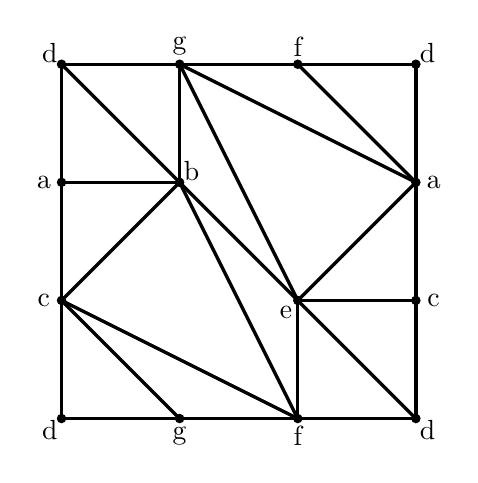
\begin{tikzpicture}[scale = .3]
    \draw[-,very thick] (0,0) -- (15,0) -- (15,15) -- (0,15) -- cycle;
    \draw[-,very thick] (0,5) -- (5,0);
    \draw[-,very thick] (0,5) -- (10,0);
    \draw[-,very thick] (0,5) -- (5,10);
    \draw[-,very thick] (0,10) -- (5,10);
    \draw[-,very thick] (0,15) -- (5,10);
    \draw[-,very thick] (5,10) -- (10,0);
    \draw[-,very thick] (5,10) -- (5,15);
    \draw[-,very thick] (5,10) -- (10,5);
    \draw[-,very thick] (5,15) -- (10,5);
    \draw[-,very thick] (5,15) -- (15,10);
    \draw[-,very thick] (10,0) -- (10,5);
    \draw[-,very thick] (10,5) -- (15,0);
    \draw[-,very thick] (10,5) -- (15,5);
    \draw[-,very thick] (10,5) -- (15,10);
    \draw[-,very thick] (10,15) -- (15,10);
    \filldraw (0,0) circle (5pt);
    \filldraw (5,0) circle (5pt);
    \filldraw (10,0) circle (5pt);
    \filldraw (15,0) circle (5pt);
    \filldraw (15,5) circle (5pt);
    \filldraw (15,10) circle (5pt);
    \filldraw (15,15) circle (5pt);
    \filldraw (10,15) circle (5pt);
    \filldraw (5,15) circle (5pt);
    \filldraw (0,15) circle (5pt);
    \filldraw (0,10) circle (5pt);
    \filldraw (0,5) circle (5pt);
    \filldraw (5,10) circle (5pt);
    \filldraw (10,5) circle (5pt);
    \node at (-.5,-.5) {d};
    \node at (5,-.75) {g};
    \node at (10,-.75) {f};
    \node at (15.5,-.5) {d};
    \node at (15.75,5) {c};
    \node at (15.75,10) {a};
    \node at (15.5,15.5) {d};
    \node at (10,15.75) {f};
    \node at (5,15.75) {g};
    \node at (-.5,15.5) {d};
    \node at (-.75,10) {a};
    \node at (-.75,5) {c};
    \node at (5.5,10.5) {b};
    \node at (9.5,4.5) {e};
  \end{tikzpicture}\\
\end{center}


%%%%%%%%%%%%%%%%%%%%%%%%%%%%%%%%%%%%%%%%%%%%%%%%%%%%%%%%%%%%%%%%%%%%%%%%%%%%%%
\begin{bibdiv}
  \begin{biblist}%[\normalsize]
    
    
    \bib{BH}{book}{
      author={Bruns, Winfried},
      author={Herzog, J\"{u}rgen},
      title={\href{https://doi.org/10.1017/CBO9780511608681}%
        {Cohen-Macaulay rings}},
      series={Cambridge Studies in Advanced Mathematics},
      volume={39},
      publisher={Cambridge University Press, Cambridge},
      date={1993},
      pages={xii+403},
      % isbn={0-521-41068-1},
      % review={\MR{1251956}},
      % doi={10.1017/CBO9780511608681},
    }
    
    \bib{Stanley}{book}{
      author={Stanley, R.P.},
      title={Combinatorics and Commutative Algebra},
      series={Progress in Mathematics},
      volume={41},
      edition={2},
      publisher={Birkh{\"a}user Boston},
      date={1996},
      pages={xi+166}
      % isbn={9780817643690},
    }
    
    \bib{MS}{book}{
      author={Miller, Ezra},
      author={Sturmfels, Bernd},
      title={Combinatorial Commutative Algebra},
      series={Graduate Texts in Mathematics},
      volume={227},
      publisher={Springer-Verlag New York},
      date={2005},
      pages={xiv+420}
      % isbn={9780387237077},
    }
    
    \bib{Peeva}{book}{
      author={Peeva, Irena},
      title={Graded Syzygies},
      series={Algebra and Applications},
      volume={14},
      publisher={Springer-Verlag London},
      date={2011},
      pages={xii+304}
      % isbn={9781447126164},
    }
    
    \bib{Munkres}{book}{,
    author={Munkres, James~R.},
    title={Elements Of Algebraic Topology},
    publisher={CRC Press},
    date={2018},
    pages={x+468}
    % isbn={9780429962462},
    }
    
    \bib{M2}{misc}{
      label={M2},
      author={Grayson, Daniel~R.},
      author={Stillman, Michael~E.},
      title={Macaulay2, a software system for research
        in algebraic geometry},
      publisher={available at \url{http://www.math.uiuc.edu/Macaulay2/}},
    }

    \bib{MFRG}{article}{
      author={\`Alvarez Montaner, Josep},
      author={Fern\'{a}ndez-Ramos, Oscar},
      author={Gimenez, Philippe},
      title={Pruned cellular free resolutions of monomial ideals},
      journal={J. Algebra},
      volume={541},
      date={2020},
      pages={126--145},
      issn={0021-8693},
      review={\MR{4014733}},
      doi={10.1016/j.jalgebra.2019.09.013},
    }

    \bib{BT}{article}{
      author={Bj\"{o}rner, Anders},
      author={Tancer, Martin},
      title={Note: Combinatorial Alexander duality---a short and elementary
        proof},
      journal={Discrete Comput. Geom.},
      volume={42},
      date={2009},
      number={4},
      pages={586--593},
      issn={0179-5376},
      review={\MR{2556456}},
      doi={10.1007/s00454-008-9102-x},
    }
    
    \bib{Cook}{article}{
      author={Cook, David, II},
      title={Simplicial decomposability},
      journal={J. Softw. Algebra Geom.},
      volume={2},
      date={2010},
      pages={20--23},
      issn={1948-7916},
      review={\MR{2881131}},
      doi={10.2140/jsag.2010.2.20},
    }
    
  \end{biblist}
\end{bibdiv}

\raggedright

\end{document}
%%%%%%%%%%%%%%%%%%%%%%%%%%%%%%%%%%%%%%%%%%%%%%%%%%%%%%%%%%%%%%%%%%%%%%
               

%%% Local Variables:
%%% mode: latex
%%% TeX-master: t
%%% End:
$t$